\documentclass{article}
\usepackage{indentfirst}
\usepackage[utf8]{inputenc}
\usepackage[margin=0.5in]{geometry}
\usepackage{graphicx}
\usepackage{verbatim}

\begin{document}

\title{Glossario di SWE}
\author{M9k}
\maketitle

%\section{TEXT}
%\subsection{TEXT}
%\subsubsection{TEXT}
%\paragraph{TEXT}
%\subparagraph{Subparagraph}Subparagraph text.\vspace{2mm}
	
\section{Glossario}
		\textbf{Progetto}\\
		Insieme di attività e compiti\\
		-per raggiungere obbiettivi con specifiche fissate\\
		-data di inizio e di fine fissate\\
		-risorse limitate (es: persone, tempo, fondi, strumenti)\\
		-consuma risorse svolgendosi\\
			
		\textbf{Processo - ISO 9000}\\
		\textit{Insieme di attività correlate} e \textit{coese} che trasformano ingressi (bisogni) in uscite (prodotti) secondo regole date, consumando risorse nel farlo\\
		Correlate: hanno un motivo/una capacità per stare assieme\\
		Coese: utili al medesimo obiettivo\\
		
		\textbf{Attività}\\
		Cosa da fare, che voglio fare, per il raggiungimento degli obbiettivi, composta da più compiti\\
		
		\textbf{Compito}\\
		Cosa che una persona deve fare, che va fatta\\

		\textbf{Fasi principali:}\\
		-Pianificazione (\textit{gestione risorse} e \textit{responsabilità})\\
		-Analisi dei requisiti (\textsl{cosa} devo fare)\\
		-Progettazione (\textit{come} farlo)\\
		-Realizzazione (con una \textit{qualità}, \textit{verificando} la correttezza, \textit{validando} i risultati)\\
		
		\textbf{Efficienza}\\
		Produttività, metrica del grado di riduzione degli sprechi\\
		Quantità prodotto realizzato/risorse utilizzate\\
		
		\textbf{Efficacia}\\
		Qualità, metrica del grado di raggiungimento degli obbiettivi interni (del fornitore) o esterni (gradimento del cliente)\\
		
		\textbf{Iterazione}\\
		Può essere anche un incremento, procedere per raffinamento o rivisitazioni (pittura)\\
		Non so se sto migliorando o meno, non quantificabile, non efficiente, rifinisco gli aspetti senza magari avanzare, non so a che punto sono\\
		
		\textbf{Incremento}\\
		Procedere per aggiunta a un impianto base (scultura)\\
		Si progredisce a punti, a baseline, quantificabile\\
		
		\textbf{Prototipo}\\
		Per provare e capire meglio, usa e getta (bozza), oppure per avere avanzamento incrementale (baseline)\\
					
		\textbf{Baseline}\\
		Prodotto prototipale, è il risultato di avanzamenti misurabili\\
		
		\textbf{Milestone}\\
		Concretizzata da almeno una baseline, punto nel tempo strategico e di riferimento, meta da raggiungere con dei risultati certi/solidi che non deve essere ritoccata (incrementali)\\
		
		\textbf{Prodotto SW}\\
		È un insieme di parti, che stanno assieme secondo la loro \textit{configurazione}.\\
		Ogni sistema fatto di parti va gestito con il \textit{controllo di configurazione}.\\
			
		\textbf{Configurazione}\\
		Modo nel quale si assemblano i pezzi di un software (ordine, parti, librerie, impostazioni, etc)\\
		Usato per il build, si gestisce con il controllo di configurazione\\
			
		\textbf{Metrica}\\
		Metodo di misurazione, l'unità di misura da sola è insignificante\\
		
		\textbf{Requisiti}\\
		1 - Condizione (capability) da chi la offre - capacità di risolvere un problema o raggiungere un obbiettivo\\
		2 - Condizione (capability) da chi la richiede - che deve essere soddisfatta o posseduta da un sistema per aderire a un obbligo (contratto, standard, specifica, documento formale)\\
		3 - Descrizione documentata di una condizione come in 1 o 2\\
		Importante siano atomici, misurabili, assegnabili a una attività, tracciabile e con un ID univoco e sensato\\
		
		\textbf{Qualifica}\\
		Verifica + Validazione\\
		\textit{Verifica}: processo di supporto, accertamento che l'esecuzione delle attività non abbia introdotto errori, rivolto ai processi, da fare per OGNI componente\\
		Per la verifica serve piano di verifica che si basa sul way of working\\
		Verifica che il codice sia verificato secondo progettazione che soddisfa requisiti\\
		\textit{Validazione}: controllo rivolto SOLO al prodotto finale, lungo e costoso, accertarsi che il prodotto realizzato corrisponda alle attese\\
		Abilitato dalle verifiche, accerta che il codice confermi i requisiti\\
		
		\textbf{Progettazione}\\
		Correttezza per costruzione, non per correzione, usa divide-et-impera per gestire complessità e ripartire le responsabilità, per produrre con efficienza ed efficacia\\
		Approccio sintetico, per capire come fare UNA soluzione (di tante possibili) soddisfacente per gli stakeholder e sufficientemente efficiente\\
		
		\textbf{Architettura - da ISO/IEC/IEEE 42010}\\
		-La decomposizione del sistema in componenti\\
		-L'organizzazione di tali componenti, definendo ruoli, responsabilità e iterazioni (chi fa cosa e come)\\
		-Le interfacce (regole strutturate) necessarie all'interazione delle componenti\\
		-I paradigmi (modo esemplare) di composizione, per fare il meglio con meno risorse possibili\\
		
		\textbf{Sistema}: aggregato di parti per un fine comune\\
		
		\textbf{Componenti}: parte di un sistema abbastanza grande da avere un ruolo specifico\\
		
		\textbf{Framework}\\
		Insieme integrato di componenti SW prefabbricate, librerie architetturali, architettura generica riusabile con buone proprietà\\
		Definite ''librerie'' prima della programmazione ad oggetti\\
		Sono bottom-up, perchè si usa codice già sviluppato (composizione e specializzazione), ma possono essere anche top-down se impongono uno stile architetturale (come scomporre il problema)\\
		Utilizzano design pattern ricorrenti\\
		
		\textbf{Design pattern architetturali}\\
		Soluzione progettuale a problema ricorrente, organizza una responsabilità architetturale lasciando alcune libertà\\
		
		\textbf{Unità}\\
		?\\
		
		\textbf{Moduli}\\
		?\\
		
		\textbf{Prove di unità}\\
		?\\
		
		\textbf{Qualità - secondo ISO 8402 e ISO 9000}\\
		Insieme delle caratteristiche di una entità che ne determinano la capacità di soddisfare esigenze espresse ed implicite, deve essere quantificabile per permettere paragoni oggettivi\\
		
		\textbf{Valutazione}\\
		Attività che si occupa di stimare\\
		
		\textbf{Sistema di qualità - secondo ISO 8402 e ISO 9000}\\
		Struttura organizzativa, responsabilità, procedure (way of working) e risorse (tempo, persone, strumenti) messe in atto per il proseguimento della qualità\\
		
		\textbf{Pianificazione della qualità - secondo ISO 9000}\\
		Le attività del sistema qualità mirate a fissare gli obiettivi di qualità, i processi e le risorse necessarie per conseguirli, per l'azienda, l'organizzazione e il progetto\\
				
		\textbf{Piano della qualità}\\
		Fissa le politiche aziendali per il perseguimento della qualità, determina gli obbiettivi di qualità del singolo processo, assume l'uso di mezzi e modalità di controllo\\
		
		\textbf{Controllo di qualità - secondo ISO 9000}\\
		Le attività del sistema qualità pianificate e attuate per assicurare che il prodotto soddisfi le attese, accertamento piuttosto che controllo\\
		
		\textbf{Standard di qualità}\\
		Raccolta organica di best practice, per evitare errori passati e idonea alla concezione e attuazione di processi di qualità assurance\\
		
		\textbf{Modelli di qualità del SW}\\
		Strumenti utili alla valutazione (dal punto di vista dell'utente/uso, della produzione/rispetto qualifica, manutenzione, portabilità e uso e della direzione/costi e benefici)\\
		Modello unico per committenti e fornitori, per uniformare la valutazione\\
		
		\textbf{ISO 9126 - Modello di definizione}\\
		-Visione esterna (relativa all'esecuzione del prodotto): funzionalità, affidabilità, efficienza, usabilità\\
		-Visione intera (relativa al prodotto non in esecuzione): manutenibilità, portabilità\\
		-Visione in uso (relativa alla percezione dell'utente o operatore)\\
		
		\textbf{ISO 14598 - Modello di valutazione}\\
		Misurazione quantitativa: scegliere una metrica per assegnare un valore, numerico o categoria, su una scala predefinita\\
		
		\textbf{ISO 25000 - 9126 + 14598 - SQuaRE}\\
		
		\textbf{Qualità di processo}\\
		Quality assurance, sistematico, per avere risultati riproducibili, identificando i momenti di verifica\\
		Usando PDCA, disposizione al miglioramento\\
		Ogni processo deve avere un controllo, non passivo, che aiuta a fissare obbiettivi metrici\\
		
		\textbf{Manuale della qualità}\\
		Documento trasversale, determinato dalla politica della qualità dell'azienda, univoca, definisce il sistema di gestione della qualità dell'organizzazione\\
		
		\textbf{CMMI: Capability Maturity Model + Integration}\\
		Strumento di valutazione della maturità dei processi dei fornitori sviluppato dal DoD\\
			
	\clearpage
	\section{Ingegneria}
		\textbf{Ingegneria}\\
			Applicazioni principi matematici e scientifici a scopo pratico, NON per esplorare nuove possibilità o espandere la scienza\\
			Mai inventare, utilizzare sempre metodi testati e funzionanti\\
			
		\textbf{Best practice}\\
		Miglior modo (way of working) per raggiungere uno scopo, secondo applicazioni passate che hanno dimostrato i risultati\\
		
		\textbf{Pratical ends}\\
		Avere un fine civile e sociale oltre che economico\\
		
	\subsection{Ingegneria del software}
		\textbf{Ingegneria del software}\\
		Disciplina per la realizzazione di \textit{prodotti software} impegnativo e che richiede collaborazione\\
		-in grande e in piccolo (tanto in quantità o poco e specializzato)\\
		-con qualità = \textit{efficacia} = grado di conformità, capacità di raggiungere gli obiettivi\\
		-con costi e tempi contenuti = \textit{efficienza} = capacità di ridurre le risorse e gli sprechi, seguendo la best practice \\
		-tutto lungo il \textit{ciclo di vita}\\
		
		\textbf{Ingegneria del software}\\
		Raccogliere, organizzare e consolidare conoscenza (body of knowledge) necessarie a realizzare progetti SW con massima efficacia e efficenza.\\
		Acquisire, utilizzare e mantenere i best practice.\\
		
		
		\textbf{Ingegneria del software}\\
		Secondo IEEE: Approccio \textit{sistematico}, \textit{disciplinato} e \textit{quantificato} allo sviluppo, uso, manutenzione e ritiro del SW.\\
		Sistematico: metodico e rigoroso, usando una metodologia precisa, per studiare ed evolvere best practice\\
		Disciplinato: regole fissate\\
		Quantificabile: efficienza ed efficacia misurabili.\\
		
		
		\textbf{Tipologie di prodotti software}\\
		-Commessa: forma, contenuto e funzioni definiti dal committente\\
		-Pacchetto: forma, contenuto e funzioni idonei alla replicazione\\
		-Componente: forma, contenuto e funzioni idonei alla composizione\\
		-Servizio: forma, contenuto e funzioni definiti dal problema\\
		
		\textbf{Le 4 P di SWE}\\
		-People (stakeholder e team di sviluppo)\\
		-Product (SW e documentazione)\\
		-Project (Insieme di attività di produzione)\\
		-Process (way of working)\\
		
		\textbf{Ciclo di vita}\\
		Insieme di stati di avanzamento del software fino al ritiro\\
		Un ciclo di vita lungo porta a elevati costi di \textit{manutenzione}\\
		
		\textbf{Manutenzione}\\
		-correttiva: fix dei bug\\
		-adattiva: rifinisco i requisiti\\
		-evolutiva: evoluzione del software secondo i nuovi usi\\
		
		\textbf{Utilità}\\
		\textit{Metrica} riguardante gli utilizzi/utenti di un prodotto nel tempo\\
		
		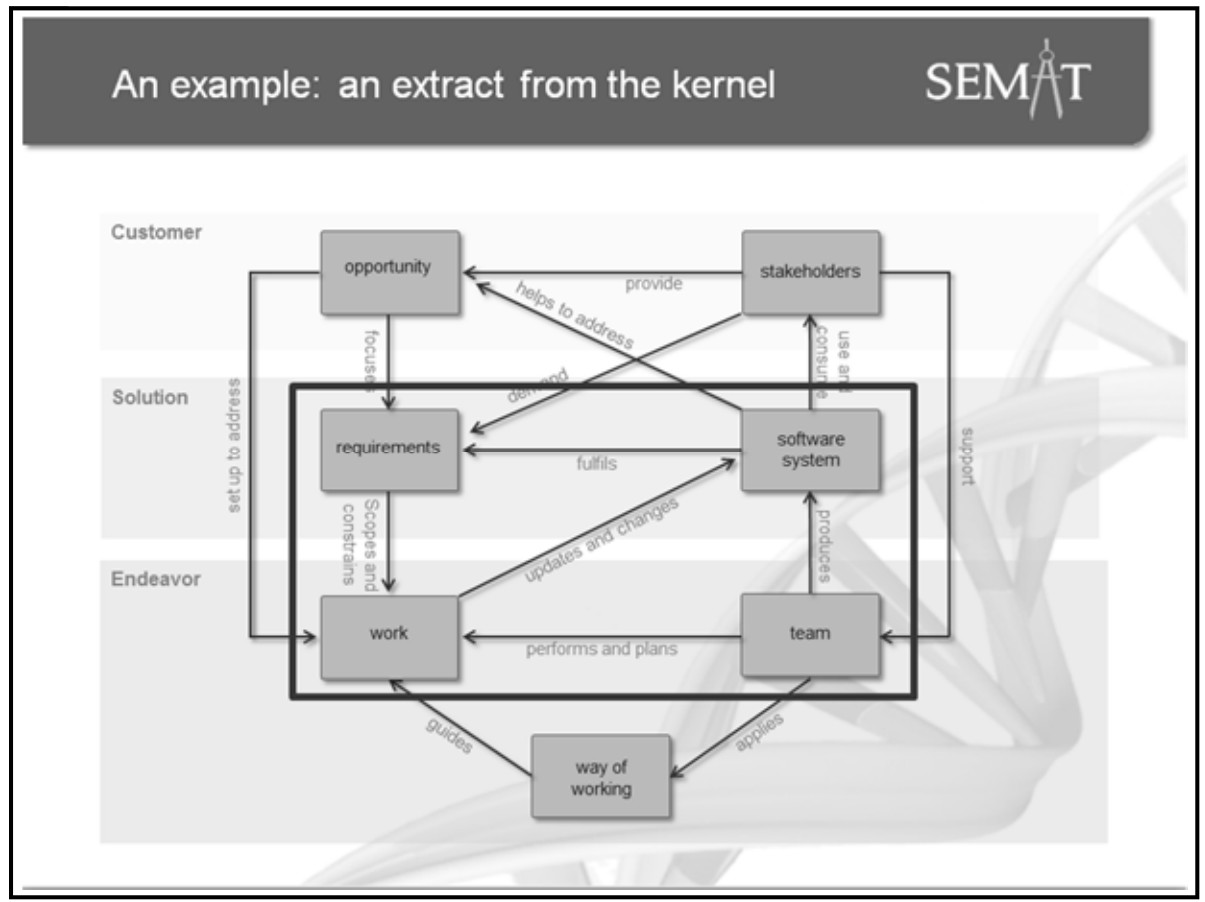
\includegraphics[width=14cm]{semat_org.jpg}\\
		
		
	\clearpage
	\section{Processi SW}
		\textbf{Ciclo di vita}\\
		Gli stati che il prodotto assume dal concepimento al ritiro\\
		Serve per valutare costi, tempi, obblighi e rischi PRIMA di svolgere il progetto\\
		Scelta tra più possibili cicli di vita, ognuno con vantaggi e limiti\\
		
		\textbf{Processi di ciclo di vita}\\
		Specificano le attività da svolgere per abilitare corrette transizioni di stato nel ciclo di vita\\
		
		
		\textbf{Modelli di ciclo di vita}\\
		Descrivono come i processi di ciclo di vita si relazionano tra di loro rispetto agli stati\\
		Aiutano a pianificare, organizzare ed eseguire lo svolgimento delle attività\\
		Svariati, scelgo in base alla situazione, ognuno con pregi e limiti\\
		
		\textbf{Ciclo di sviluppo}\\
		Ciclo di vita fino alla consegna, senza utilizzo, manutenzione e ritiro\\
		
		\textbf{Visione a grafi}\\
		Gli stati sono i nodi (concezione, sviluppo, utilizzo, ritiro, etc), gli archi le attività svolte sul prodotto necessarie per farlo avanzare.\\
		Natura degli stati e pre- e post- condizione determinate da \textit{obblighi} (vincoli contrattuali), \textit{regole} (standard di processo) e \textit{strategie}\\
		
		\textbf{Modelli più significativi}\\
		-Sequenziale o a cascata (waterfall)\\
		-Incrementale\\
		-A evoluzioni successive\\
		-A spirale\\
		-Per componenti\\
		-Agile\\
		
		\textbf{Riuso}\\
		-Occasionale: copia-incolla, basso costo, scarso impatto, da evitare\\
		-Sistematico: per progetto/prodotto/azienda, maggior costo, maggior impatto\\
		
		\textbf{Malleabilità}\\
		Un buon software non è statico, ma si modifica e si addatta in quanto usandolo si scoprono migliorie e/o cambiano gli usi\\
			
		\textbf{Processo - ISO 9000}\\
		\textit{Insieme di attività correlate} e \textit{coese} che trasformano ingressi (bisogni) in uscite (prodotti) secondo regole date, consumando risorse nel farlo\\
		Correlate: sono collegate, hanno la capacità di stare assieme\\
		Coese: hanno un motivo di stare assieme\\
		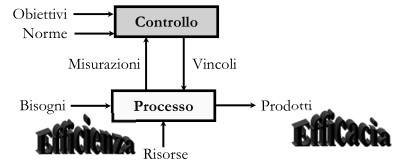
\includegraphics[width=14cm]{processi.jpg}\\
		Risorse: efficienza = produttività, cosa ho fatto/quante risorse ho utilizzato\\
		Misurazione: efficacia, raggiungimento di obbiettivi interni (del fornitore, cioè di chi crea il software) o esterni (gradimento da parte del cliente)\\
		
		\textbf{Economicità}\\
		Insieme di efficienza ed efficacia, da controllare DURANTE lo sviluppo usando:\\
		-dati tempestivi (non si può attendere la fine, sarebbe troppo tardi)\\
		-dati accurati (niente opinioni personali ma numeri)\\
		-non intrusività (non bloccare il lavoro per controllare il progresso)\\

		\textbf{Standard di processo}\\
		Voluti dai committenti per vincolare il fornitore\\
		Per facilitare \textit{controllo}, \textit{collaudo} e \textit{accettazione}, indipendenti dal modello del ciclo di vita\\
		Settoriali o generali/trasversali\\
		Vincolo (imposto) o riferimento (non imposto, come modello)\\
		
		\textbf{Standard come modello di azione}\\
		Sono una serie di passaggi da compiere, guida passo a passo, come una ricetta\\
		Definizione e imposizione di \textit{procedure}, definizione e proposizione di \textit{processi da specializzare}\\
		
		\textbf{Standard come modello di valutazione}\\
		Servono per avere una valutazione sul comportamento del progetto\\
		Modelli più generali, copre più contesti, per identificare best practice\\
	
		\textbf{ISO/IEC 12207:1995}\\
		Letta come 12 207\\
		Più diffuso, ad alto livello, molto astratto, preso spunto dagli standard militari del dipartimento di difesa\\
		Identifica i processi di ciclo di vita del SW\\
		Struttura modulare che richiede specializzazione\\
		Specifica le responsabilità sui processi e i prodotti\\
		Tre parti principali: processi primari, di supporto e organizzativi\\
	
		\textbf{Processi primari}\\
		Necessari per l'esistenza di un progetto\\
		-Acquisizione (gestione dei sotto-fornitori)\\
		-Fornitura (gestione rapporti con il cliente, primo passo di un progetto)\\
		-Sviluppo\\
		-Gestione operativa (utilizzo, erogazione, installazione)\\
		-Manutenzione (correzione, adattamento, evoluzione)\\
		
		\textbf{Processi di supporto}\\
		-Documentazione\\
		-Accertamento qualità\\
		-Gestione delle versioni e delle configurazioni\\
		-Qualifica: verifica + validazione\\
		-Revisioni congiunte con il cliente\\
		-Verifiche ispettive interne\\
		-Risoluzione dei problemi (gestione dei cambiamenti)\\
		
		\textbf{Processi organizzativi}\\
		-Gestione dei processi\\
		-Gestione delle infrastrutture\\
		-Miglioramento del processo\\
		-Formazione personale\\
		
		\textbf{Tecniche}\\
		Ricette per svolgere determinati compiti\\
		Vincoli o strategie restringono il grado di libertà\\
		
		\textbf{Buona organizzazione}\\
		Si basa sul riconoscere i processi, adottarli consapevolmente ed efficacemente e supportarli in modo efficiente\\
		
		\begin{comment}
			\textbf{Tipi di processo}\\
			-Standard: di base, generico, condiviso tra aziende nello stesso dominio applicativo\\
			-Definito: specializzazione per adeguare un processo standard a caratteristiche aziendali\\
			-Di progetto: istanziato, usano risorse aziendali per raggiungere obbiettivi prefissati e con tempo limitato (progetti)\\
			
			\textbf{Processi specializzati/definiti}\\
			-Chiari, stabili, documentati\\
			-indipendenti dal modello di ciclo di vita adottato\\
			-Indipendenti dalle tecnologie\\
			-Indipendenti dal dominio applicativo\\
			-Indipendenti dalla documentazione richiesta\\
			
			\textbf{Processi di progetto}\\
			-Ben pianificati\\
			-Chiare scelte di specializzazione (definire lo scenario, le attività e i compiti aggiuntivi e specifici, organizzare le relazione tra i processi specializzati)\\
			-Massima attenzione nel condurre il progetto\\
			-Valutazione critica dell'esito (formalizzare le parti che operano bene)\\
			
			\textbf{Dipendono da:}\\
			-Dimensione del progetto\\
			-Complessità del progetto\\
			-Rischi identificati (da dominio applicativo e tecnologie)\\
			-Competenze ed esperienza delle risorse umane\\
			-Fattori dipendenti dal contratto\\
		\end{comment}
		
		\textbf{Organizzazione interna - Verifica qualità del processo}\\
		Ciclo PDCA o ciclo di Deming:\\
		-Plan: definire le strategie per attività, scadenze, responsabilità e risorse per raggiungere determinati obbiettivi\\
		-Do: eseguire secondo i piani\\
		-Check: verificare l'esito delle azioni rispetto le attese\\
		-Act: applicare soluzioni correttive alle carenze o consolidamento delle strategie efficaci\\
		
		\textbf{Processi e modelli di ciclo di vita}\\
		-La specifica dei processi non determina il modello di ciclo di vita\\
		-Il livello di coinvolgimento del cliente determina natura, funzione e sequenza dei processi di revisione\\
		-Quando il SW è parte di un sistema complesso il modello di ciclo di vita a \textit{livello di sistema} è spesso sequenziale.\\
		
		\textbf{Influenze sul modello di ciclo di vita}\\
		-Politiche di acquisizione e di sviluppo (versione unica o multipla, dipendenza da/verso altre componenti)\\
		-Natura, funzione e sequenza dei processi di revisione (interne, esterne, non bloccanti)\\
		-Necessità/utilità di fornire evidenze preliminari di fattibilità (prototipi bozza o baseline, studi e analisi preliminari)\\
		-Esigenza di iterazioni o di configurazioni (build, deployment)\\
		-L'evoluzione del sistema e dei suoi requisiti, che	porta a iterazioni\\
			
			
			
	\clearpage
	\section{Ciclo di vita}
	
		\textbf{Stati principali}\\
		-Concezione\\
		-Sviluppo\\
		-Utilizzo\\
		-Ritiro\\
		
		\textbf{Organizzare le attività di processo}\\
		Si devono identificare dipendenze tra ingressi ed uscite, poi fissarle nel tempo assieme ai criteri di attivazione (pre-condizioni) e di completamento (post-condizioni)\\
		
		\textbf{Fase}\\
		Stazionamento in uno stato del ciclo di vita o in una transizione tra stati\\
		
		\textbf{Sistema di qualità}\\
		Associato al modello per assicurare conformità e maturità\\
		
		
		\textbf{Modello a cascata o sequenziale}\\
		Fasi:\\
		-Analisi (requisiti di sistema e software, etc)\\
		-Progettazione (Design, etc)\\
		-Realizzazione (Codifica, integrazione, collaudo, etc)\\
		-Manutenzione\\
		Eseguite in modo rigidamente sequenziale, no parallelismo, guidato da documentazione, codice solo alla fine, con pre-condizioni e post-condizioni per ogni fase\\
		Eccessiva rigidità, non permette modifiche ai requisiti, necessita di molta manutenzione, molto burocratico e poco realistico\\
		Big-gan integration: si integra tutto alla fine in un solo colpo, se non funziona difficile isolare e correggere il problema\\
		\textbf{Correzioni}\\
		-Prototipazione: usa e getta, scrivendo la documentazione si fanno delle prove\\
		-Cascata con ritorni: torno indietro per correggere/rifare una parte, rompendo il modello, iterazioni! - Modello iterativo\\
		Segue un approccio \textit{predittivo}, fissati i piani e devono essere rispettati\\
		
		\textbf{Modello iterativo}\\
		Applicabile a qualsiasi altro modello, consente l'adattamento (a evoluzione dei problemi, requisiti, soluzioni e tecnologie)\\
		Si ritorna indietro rispetto l'asse temporale\\
		
		\textbf{Modello incrementale}\\
		Fasi:\\
		-Define outline requiments (schema generale)\\
		-Assign requiments to increments (essenziale per poter procedere a incrementi)\\
		-Design system architecture (come le parti si compongono, essenziale per il parallelismo)\\
		finchè non ho il sistema finale:\\
		|-Develop system increment\\
		|-Validate increment\\
		|-Integrate increment\\
		|-Validate system\\
		Possibile svolgere gli incrementi in parallelo\\
		Riassumibile in : ``Analisi e progettazione'', poi ciclo su ``Progettazione di dettaglio'' e ``Implementazione dettaglio''\\
		Segue un approccio \textit{adattivo}, si riescono a effettuare dei cambiamenti\\
		
		\textbf{Modello evolutivo (incrementale)}\\
		Per uno scenario che varia (es Browser), molteplici versioni intermedie, ogni fase ammette iterazioni multiple e parallele\\
		Si basa su una analisi iniziale, poi cicla su analisi e progettazione ed sviluppo e validazione\\
		
		\textbf{Modello a componenti}\\
		Si basa sul riutilizzo di componenti\\
		Fasi:\\
		-Analisi requisiti\\
		-Analisi componenti\\
		-Adattamento dei requisiti (controllo cosa fa al caso mio e come dovrò modificarlo per soddisfare i requisiti)\\
		-Progettazione con riuso\\
		-Sviluppo e integrazione\\
		-Validazione di sistema\\
		
		\textbf{Modelli agili}\\
		-Niente regole rigide\\
		-Il software funzionante è più importante di una buona documentazione\\
		-Collaborare con il cliente, non negoziare\\
		-Essere reattivi, non mirare alla pianificazione\\
		Ma:\\
		-Adattare le regole è ok, ma bisogna mantenere un occhio su costi/benefici\\
		-La mancanza della documentazione fa lievitare il costo di manutenzione\\
		-Non pianificare significa non sapere se si sta avanzando e i rischi che si corrono\\
		\textbf{User story}\\
		Minuta, resoconto con il cliente, dialogando specifica i problemi e i requisiti, pezzo per pezzo\\
		Sarà una lista di cose che vuole, che preferirebbe e che non vuole, da usare per controllare l'avanzamento e l'efficacia\\
		\textbf{3 forme principali}\\
		La maggiore: \textbf{SCRUMB}\\
		Iterazione controllata, c'è un \textit{backlog} di cose da svolgere, si sceglie quali fare (\textit{sprint}) prendendo le più utili/necessarie/importanti, le faccio, le unisco in un incremento e itero nuovamente\\
		Sprint usualmente di circa 2 settimane, con misurazioni giornaliere brevi di tipo stand-up, intrusive!\\
		
		\textbf{Il ciclo di vita secondo SEMAT}\\
		Sequenza di punti/indicazioni suddivisi per categoria per aiutare a organizzare/misurare/controllare l'avanzamento e l'aver completato le principali problematiche durante tutto il ciclo di vita\\
		
		
	\clearpage
	\section{Gestione di progetto}
		\textbf{Fondamenti}\\
		Gestione di progetto - è un processo organizzativo per gestire altre attività\\
		-Processi di progetto istanziati da processi aziendali, a loro volta istanziati da standard di processo\\
		-Per stimare costi e le risorse necessarie\\
		-Per \textit{pianificare} attività ed assegnarle alle persone, in modo sistematico, disciplinato e quantificabile usando best practice\\
		-Controllare le attività e verificare i risultati per prendere provvedimenti\\
		-Assegnare le attività alle persone\\
		
		\textbf{Funzione}\\
		Funzione aziendale, fissa, tra sviluppo, direzione (decisioni), amministrazione (gestione del supporto ai progetti), qualità (economicità)\\
		
		\textbf{Ruolo}\\
		Ruolo in un progetto, assegnato in base alla propria funzione\\
		
		\textbf{Ruolo: analista}\\
		Devono capire il problema e i requisiti/\textit{cosa fare}, pochi, competenze sul dominio del problema, grande influenza, presenti solo all'inizio\\
		Devono anche fare l'analisi di fattibilità\\
		
		\textbf{Ruolo: progettista}\\
		Deve capire \textit{come risolvere il problema}, attraverso la soluzione migliore come economicità, pochi, competenze sulle tecnologie, influenza sulle scelte tecniche e tecnologiche, a volte seguono il progetto fino alla manutenzione\\
		
		\textbf{Ruolo: programmatore}\\
		Molti, competenze tecniche, visione e responsabilità circoscritte, realizzano e mantengono il prodotto deciso dal progettista\\
		
		\textbf{Ruolo: responsabile}\\
		Aggrega i ruoli e li fa cooperare\\
		Responsabilità su pianificazione, gestione delle risorse umane, controllo e relazioni esterne\\
		Capacità tecniche necessarie per valutare rischi, scelte ed alternative\\
		
		\textbf{Ruolo: amministratore}\\
		Controllo ambiente di lavoro, responsabile dell'efficienza, amministrazione delle infrastrutture di supporto, risoluzione problemi riguardanti la gestione dei processi, gestione della documentazione, controllo di versioni e configurazione\\
		Funzione o ruolo nel progetto, dipende dalla organizzazione aziendale\\
		
		\textbf{Ruolo: verificatore}\\
		Gestiscono verifiche e validazioni, capacità di giudizio e relazione, competenze tecniche, esperienza professionale e conoscenza delle norme, sempre presenti\\
		
		\textbf{Ruolo: gestione qualità}\\
		Funzione aziendale, non ruolo, gestisce way of working aziendale\\
		Richiede applicazione rigorosa dei processi adottati, mantiene il ciclo PDCA, si assicura della sufficienza della qualità verso il committente e verso la direzione\\
		
		\subsection{Pianificazione di progetto - compito del Responsabile}
			Con l'aiuto di strumenti, definizione delle attività per:\\
			-Pianificare lo svolgimento e controllarne l'attuazione\\
			-Avere una base per gestire l'allocazione delle risorse\\
			-Stimare e controllare scadenze e costi\\
			
			Svolgimento:\\
			-Identificazione della lista delle attività\\
			-Disposizione in ordine delle attività secondo le dipendenze\\
			-Stima delle risorse per attività\\
			-Allocazione del personale rispettando i vincoli (ore giornaliere, competenze, etc)\\
			-Creazione dei diagrammi del progetto, se qualcosa non va bene torno alla stima\\
			
			Realizzato con:\\
			-Diagrammi di Gantt\\
			-PERT\\
			-WBS\\
			
			\textbf{Gantt}\\
			Dislocazione temporale delle attività pianificate e eseguite, per controllare le stime con i progressi\\
			Utilizzabile anche con le persone per controllare sovrapposizioni o lavori in gruppo\\
			
			\textbf{PERT}\\
			Sottolinea dipendenze temporali tra le attività, per ragionare sulle scadenze, evidenzia il cammino critico (quello con slack minore o =0) e i vari slack (margine)\\
			
			\textbf{WBS}\\
			Struttura gerarchica delle attività, evidenzia le sotto-attività univocamente identificate, anche non sequenziali\\
			
			\textbf{Allocazione su più progetti}\\
			Risorse allocate in più processi per evitare sotto-utilizzo e richieste dei clienti, producono cammini critici\\
			
			\textbf{Stima costi di progetto}\\
			Definire durata in ore di lavoro e costo stimandolo secondo esperienza, analogia, competizione o algoritmo predittivo (non preciso), poi rapportandolo alle ore di calendario\\
			
			\textbf{Piano di progetto}\\
			Va documentato, si indica anche come si è giunti alla stima delle risorse necessarie\\
			Scritto dal responsabile, letto da verificatore e stakeholders, poi passato al team\\
			Contenuti:\\
			-risorse disponibili e le loro assegnazione alle attività\\
			-scansione delle attività nel tempo\\
			Obiettivi:\\
			-Organizzare le attività con efficienza\\
			-Facilitare la misurazione di avanzamento fissando \textit{milestone}\\
			Struttura tipica:\\
			-Introduzione (scopo e struttura)\\
			-Organizzazione del progetto\\
			-\textbf{Analisi dei rischi} - qualsiasi evento imprevisto fa modificare il piano di progetto, meglio prevedere\\
			-Risorse disponibili\\
			-Suddivisione del lavoro\\
			-Calendario delle attività\\
			-Meccanismi di controllo e rendicontazione\\
			
			\textbf{Rischi}\\
			-Sforare i tempi/budget\\
			-Risultati insoddisfacenti\\
			Motivi:\\
			-Tecnologie di lavoro\\
			-Rapporti interpersonali\\
			-Organizzazione del lavoro\\
			-Requisiti e rapporti con gli stakeholder\\
			-Tempi e costi\\
		
			\textbf{Gestione dei rischi}\\
			Durante la pianificazione, sempre sotto gestione del progetto\\
			-Identificazione (in qualsiasi ambito, di qualsiasi tipo)\\
			-Analisi (probabilità che accadano e il livello di impatto)\\
			-Pianificazione (come mitigare o evitare)\\
			-Controllo (durante tutto lo svolgimento, con misurazioni, per raffinare le strategie e modificare la lista dei rischi identificati)\\
			Pianificando su vincoli lunghi ma in periodi brevi ho errori minori\\
			
			\textbf{Baseline}\\
			Prodotto prototipale, è il risultato di avanzamenti misurabili\\
			
			\textbf{Milestone}\\
			Concretizzata da almeno una baseline, punto nel tempo strategico e di riferimento, meta da raggiungere con dei risultati certi/solidi che non deve essere ritoccata (incrementali)\\
			Requisiti per buoni milestone:\\
			-specifiche per obbiettivi\\
			-delimitate per ampiezza ed ambizioni, raggiungibili\\
			-incrementali e misurabili come impegno necessario\\
			-coerenti con la strategia di progetto\\
			-traducibili in compiti assegnabili\\
			-puntuali\\
			-dimostrabili agli stakeholder\\
			
			\textbf{Tempo persona}\\
			Diverso dal tempo di calendario, influenzato da efficacia ed efficenza, difficile da valutare\\
		
	\clearpage
	\section{Amministrazione} 
		\textbf{Amministrazione di sistema}\\
		Equipaggiare, organizzare e gestire l'ambiente di lavoro e di produzione, a supporto dei processi istanziati dai processi, scelte tecnologiche concordate, no scelte gestionali\\
		-Reperimento, gestione, organizzazione e manutenzione di risorse informatiche e di servizi\\
		-Gestione del controllo di versione\\
		-Gestione della configurazione, del build e dei test e validazioni automatici\\
		-Gestione dei documenti\\
		-Gestione dell'ambiente di lavoro\\
		-Redazione e manutenzione di regole e procedure di lavoro - \textit{norme}\\
		
		\textbf{Issues o ticket}\\
		Idea, questione, problema, attività, etc, considerabile in due modi:\\
		-in avanti: compito, c'è una attività da fare, che posso scegliere e svolgerla, oppure che qualcuno sceglie per me pianificando, in base a un ordine di priorità\\
		-all'indietro: cosa da fare o considerare, qualcuno deve gestirlo\\
		
	\clearpage
	\section{Analisi dei requisiti}
		\textbf{Requisiti secondo IEEE}\\
		1 - Condizione (capability) da chi la offre - capacità di risolvere un problema o raggiungere un obbiettivo\\
		2 - Condizione (capability) da chi la richiede - che deve essere soddisfatta o posseduta da un sistema per aderire a un obbligo (contratto, standard, specifica, documento formale)\\
		3 - Descrizione documentata di una condizione come in 1 o 2\\
		Importante siano atomici, misurabili, assegnabili a una attività, tracciabile e con un ID univoco e sensato\\
		
		\textbf{Qualifica}\\
		Verifica + Validazione\\
		\textit{Verifica}: processo di supporto, accertamento che l'esecuzione delle attività non abbia introdotto errori, rivolto ai processi, da fare per OGNI componente\\
		Per la verifica serve piano di verifica che si basa sul way of working\\
		Verifica che il codice sia verificato secondo progettazione che soddisfa requisiti\\
		\textit{Validazione}: controllo rivolto SOLO al prodotto finale, lungo e costoso, accertarsi che il prodotto realizzato corrisponda alle attese\\
		Abilitato dalle verifiche, accerta che il codice confermi i requisiti\\
		
		\textbf{Analisi}\\
		-Studio dei bisogni e delle fonti del dominio applicativo\\
		-Prima classificazione dei requisiti\\
		-Modellazione concettuale del sistema - secondo gli use case\\
		-Assegnazione dei requisiti a parti distinte del sistema - secondo gli use case\\
		-Negoziazione con il committente, consolidamento della classificazione dei requisiti (l'ordine di importanza)\\
		
		\textbf{Piano di qualifica}\\
		-Definizione delle strategie di verifica\\
		-Metodi, tecniche e procedure da usare per la validazione\\
	
		\textbf{Attività di analisi}\\
		-Studiare e definire il problema\\
		|-Identificare il prodotto da commissionare (compito del cliente)\\
		|-Capire cosa realizzare (cliente + fornitore)\\
		|-Definire gli accordi contrattuali (cliente + fornitore)\\
		-Verificare le implicazioni di costo e di qualità\\
		|-Requisiti espliciti o impliciti, diretti o derivati per la soddisfazione del cliente\\
		-Studio dei bisogni e delle fonti (\textit{identificare}, \textit{specificare} e \textit{classificare} i requisiti dal punto di vista committente e conoscendo l'ambito)\\
		|-identificare: precisamente, che requisito serve\\
		|-specificare: secondo quali limitazioni/regole\\
		|-classificare: capirne l'importanza o la negoziabilità\\
		-Modellazione concettuale del sistema\\
		|-Partizionamento in componenti per l'allocazione dei requisiti, con diagramma dei casi d'uso (analisi - cosa, non il come)\\
		-Ripartizione dei requisiti a parti del sistema\\
		-Accertarsi della soddisfacibilità dei requisiti\\
		-Assicurarsi che i requisiti concordati siano solo e tutti quelli necessari e sufficienti\\
		-Determinare con il cliente l'utilità strategica\\
		
		\textbf{Documentazione - processo di supporto}\\
		-Definizione dei bisogni (utente - contrattuali, il cosa e SW - il come)\\
		Analisi di fattibilità - del fornitore, riservato, da fare velocemente per considerare se partecipare all'appalto\\
		Analisi dei requisiti - documento contrattuale, sostituisce il capitolato\\
		
		\textbf{Gestione del prodotto - processo di supporto}\\
		-Tracciamento requisiti (sapere da che esigenza arrivano)\\
		-Impostazione e configurazione della configurazione - con versioning, automatizzata\\
		-Gestione dei cambiamenti (discuterli, capirli e motivarli, sempre con delle regole)\\
		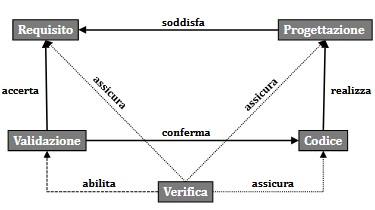
\includegraphics[width=10cm]{verifica.jpg}\\
		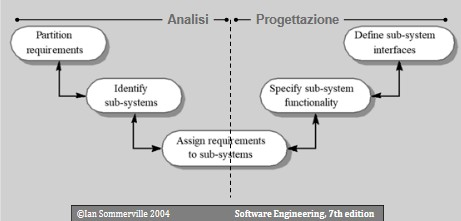
\includegraphics[width=10cm]{analisi_progettazione.jpg}\\
		
		\textbf{Approccio funzionale}\\
		Penso all'obbiettivo, lo divido in parti e sottoparti, decomposizione, istintivo ma scomodo\\
		Top-down - programmazione procedurale\\
		
		\textbf{Approccio object-oriented}\\
		Inizio dal generico astratto e specializzo estendendo, permesso dalle interfacce, i problemi li correggo solo una volta in alto, favorisce riutilizzo\\
		Analisi dei requisiti in formalismi grafici (diagramma dei casi d'uso)\\
		Bottom-up, aggregazione di parti, design pattern e riutilizzo, programmazione ad oggetti\\
		
		\textbf{Approccio con modello agile}\\
		Si deve continuare a ciclare l'analisi per rifinire i requisiti e quindi il backlog\\
		
		\textbf{Decidere o meno di proseguire}\\
		-Rapporto costi benefici (nel mercato attuale e quello futuro)\\
		-Individuare rischi (complessità e incertezze)\\
		-Fattibilità (tecnologiche, conoscenza, formazione)\\
		-Valutazione delle scadenze temporali\\
		-Valutare alternative:\\
		|-Scelte architetturali come sistema decentralizzato, client-server, etc)\\
		|-Strategie realizzative: riuso o sviluppo da zero\\
		|-Strategie operative: Avvio, esercizio, manutenzione del sistema e formazione utenti\\
		
		\textbf{Analisi dei requisiti - metodologie}\\
		-Mi pongo nei panni del cliente, per capire le cose implicite secondo lui\\
		-Interagisco con il cliente/committente, interviste, poi faccio minuta di riunione (forma sintetica) approvata da entrambe le parti\\
		-Brainstorming, idee senza ordine, in modo creativo (necessito di qualcuno che scriva e qualcuno che regoli)\\
		-Prototipazione interna o esterna, da discutere con il cliente\\
		
		\textbf{Classificazione dei requisiti}\\
		Per fare ordine, per poterli ritrovare e per essere sicuri di non saltarne una parte\\
		-\textit{Requisi/attributi del prodotto}: cosa devo fare\\
		-\textit{Requisi/attributi di processo}: come devo fare, way of working, chi paga può deciderlo\\
		
		\textbf{Esempio di classificazione dei requisiti}\\
		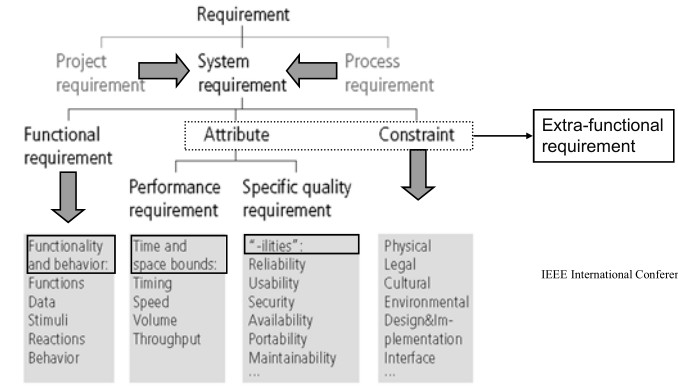
\includegraphics[width=10cm]{classificazione_requisiti.jpg}\\
		
		
		\textbf{Classificazione per utilità strategica dei requisiti}\\
		-Obbligatori: irrinunciabili\\
		-Desiderabili: con valore aggiuntivo riconoscibile\\
		-Opzionali: relativamente utili o contrattabili più avanti\\
		
		\textbf{Specifica del progetto - secondo IEEE 830-1998}\\
		Deve essere:\\
		-Priva di ambiguità\\
		-Corretta\\
		-Completa\\
		-Verificabile\\
		-Consistente\\
		-Modificabile\\
		-Tracciabile\\
		-Ordinata per rilevanza\\
		
		Parti:\\
		-Introduzione (scopo documento e del progetto, glossario, riferimenti normativi e non, struttura del documento)\\
		-Descrizione generale (prospettive, funzioni del prodotto, caratteristiche degli utenti, vincoli, assunzioni e dipendenze)\\
		-Specifica requisiti (definizione requisiti utente e di sistema, prima composizione del sistema, evoluzione attesa del sistema)\\
		-Eventuali appendici\\
		
		Scritta in formato formale o semi-formale, con diagrammi e formule, ricercando chiarezza espressiva, strutturale (separare requisiti funzionali e non) ed atomicità e aggregazione (requisiti elementari, correlazioni chiare)\\
		
		\textbf{Verifica dei requisiti}\\
		Eseguita su un documento organizzato, non posso eseguire test pratici essendo documentazione, tramite due approcci:\\
		-Walkthrought: si controlla tutto, non so dove sono i problemi e come identificarli, lenta e costosa\\
		-Ispezione: ho una checklist di indicatori di possibili problemi, scorro il documento, se ne rilevo approfondisco il controllo, più veloce\\
		
		\textbf{Classificazione}\\
		Con ID risulta scomodo, usare numerazione gerarchica sequenziale basato sulla struttura del documento (es 2.7.2) o coppie -categoria, numero-\\
		Classificati con strumenti, NON a mano, per mantenere automatico il propagarsi dei cambiamenti tra requisito, parte della specifica e componente del sistema\\
		
		\textbf{Riuso}\\
		Progettazione influenzabile da esigenza o opportunità di riuso di:\\
		-componenti aziendali preesistenti\\
		-componenti commerciali\\
		-componenti imposte dal cliente\\
		
		\textbf{Milestone per l'analisi dei requisiti secondo SEMAT} \\
		-\textbf{Conceived}: committente e stakeholder hanno la necessità di avere un prodotto SW, hanno un bisogno\\
		-\textbf{Bounded}: Il fornitore fissa i bisogni macro e i meccanismi di gestione dei requisiti\\
		-\textbf{Coherent}: Il fornitore ha classificato i requisiti, quelli essenziali sono chiari e ben definiti\\
		-\textbf{Acceptable}: I requisiti fissati definiscono un sistema soddisfacente per gli stakeholder (il fornitore chiede e ha l'approvazione)\\
		-\textbf{Addressed}: Secondo il fornitore il prodotto soddisfa i principali requisiti, possibile il rilascio e l'uso\\
		-\textbf{Fulfilled}: Gli stakeholder confermano che il prodotto soddisfa abbastanza requisiti da avere la piena approvazione\\
		
		
		
	\clearpage
	\section{Progettazione}
		\textbf{Progettazione}\\
		Correttezza per costruzione, non per correzione, usa divide-et-impera per gestire complessità e ripartire le responsabilità, per produrre con efficienza ed efficacia\\
		Approccio sintetico, per capire come fare UNA soluzione (di tante possibili) soddisfacente per gli stakeholder e sufficientemente efficiente\\
		Input: i requisiti da analisi dei requisiti, che ha adottato un approccio investigativo, con il massimo approfondimento possibile\\
		Prodotti: documentazione sull'architettura e i suoi modelli logici, definendo l'architettura\\
		
		\textbf{Responsabilità - secondo Dijkstra}\\
		-Analisi dei requisiti: Definire le proprietà/requisiti in modo da soddisfare le necessità\\
		-Progettazione: Garantire una soluzione economica che ha i requisiti individuati\\
		-Codifica: Produrre il SW secondo la progettazione\\
		
		\textbf{Architettura - da ISO/IEC/IEEE 42010}\\
		-La decomposizione del sistema in componenti\\
		-L'organizzazione di tali componenti, definendo ruoli, responsabilità e iterazioni (chi fa cosa e come)\\
		-Le interfacce (regole strutturate) necessarie all'interazione delle componenti\\
		-I paradigmi (modo esemplare) di composizione, per fare il meglio con meno risorse possibili\\
		
		\textit{Sistema}: aggregato di parti per un fine comune\\
		\textit{Componenti}: parte di un sistema abbastanza grande da avere un ruolo specifico\\
		
		Esistono più stili, aderendo a uno si garantisce coerenza e consistenza\\
		
		\textbf{Qualità di una buona architettura}\\
		-Sufficienza: capacità di soddisfare TUTTI i requisti\\
		-Comprensibilità: anche per gli stakeholder, per dimostrare gli avanzamenti\\
		-Modularità: suddivisa in parti chiare e ben distinte secondo un criterio, ci sono due strade per farlo:\\
		|-Suddividere in blocchi logici\\
		|-Information hiding - in caso di cambiamenti ci sono meno perturbazioni interne\\
		-Robustezza: supporto ad errori dell'utente e dell'ambiente\\
		-Flessibilità: permette modifiche a costo contenuto al variare dei requisiti\\
		-Riusabilità: se sue parti possono essere usate in altre applicazioni\\
		-Efficienza: nel tempo, spazio e comunicazioni\\
		-Affidabilità: altamente probabile che svolga bene il suo compito quando utilizzata, non si blocca se qualcosa fallisce\\
		-Disponibilità: la manutenzione di una parte non deve bloccare tutto il sistema a lungo (o non farlo)\\
		-Sicurezza rispetto a malfunzionamenti: grado di ridondanza\\
		-Sicurezza rispetto a intrusioni\\
		-Semplicità: ogni parte ha il necessario e niente di superfluo, semplice ma non semplificato\\
		-Incapsulazione (information hiding): L'interno non è visibile dall'esterno, solo l'interfaccia visibile, migliora manutenibilità, riutilizzo ed impedisce assunzioni sull'interno\\
		-Coesione: le parti che stanno assieme hanno lo stesso obbiettivo, motivo, ruolo\\
		|-Secondo diverse categorizzazioni (funzionale, sequenziale, informativa, etc), migliore quella che predilige information hiding\\
		-Basso accoppiamento: le parti distinte dipendono poco o nulla tra di loro (VEDERE SOTTO)\\
		
		\textbf{Qualità: Accoppiamento}\\
		Parti diverse possono essere dipendenti tra di loro in modo errato\\
		MAI basarsi su assunzioni dell'interno di altre classi, non imporre vincoli dall'esterno verso l'interno di altre parti, condividere frammenti delle stesse risorse/dati\\
		Accoppiamento necessario, se le parti non comunicano non è un sistema, ma da tenere basso\\
		Metriche: M componenti, U grado di utilizzo reciproco\\
		U minimo insieme vuoto, massimo M x M\\
		\textit{SFIN} = Fan-IN Strutturale = indice di utilità, quante volte una componente è utilizzata, da massimizzare\\
		\textit{SFOUT} = Fan-OUT Strutturale = indice di dipendenza, quante componenti viene utilizzata dalla mia, da minimizzare\\
		
		\textbf{Progettazione architetturale}\\
		Di tre tipi:\\
		-top-down, stile funzionale, decomposizione dei problemi\\
		-bottom-up, orientato agli oggetti, composizione e specializzazione\\
		-meet-in-the-middle, intermedio, più usato, il problema viene scomposto ed analizzato, poi si costruisce per composizione e specializzazione\\
		
		\textbf{Framework}\\
		Insieme integrato di componenti SW prefabbricate, librerie architetturali, architettura generica riusabile con buone proprietà\\
		Definite ''librerie'' prima della programmazione ad oggetti\\
		Sono bottom-up, perchè si usa codice già sviluppato (composizione e specializzazione), ma possono essere anche top-down se impongono uno stile architetturale (come scomporre il problema)\\
		Utilizzano design pattern ricorrenti\\
		
		\textbf{Design pattern architetturali}\\
		Soluzione progettuale a problema ricorrente, organizza una responsabilità architetturale lasciando alcune libertà\\
		
		\textbf{Pattern architetturali}\\
		-Architettura multilivello\\
		Come OSI e TPC/IP\\
		-Architettura three-tier, a livelli\\
		GUI, logica operativa (business logic) e organizzazione dei dati (DBMS)\\
		-Architettura produttore-consumatore\\
		Collaborazione su pipeline\\
		
		\textbf{Progettazione di dettaglio}\\
		Attività:\\
		-definizioni dei moduli/\textbf{unità} realizzative: realizzabili da un singolo programmatore, corrisponde a funzionalità o responsabilità ben definita\\
		-Specifica delle unità come insieme di \textbf{moduli}: dipende dal linguaggio di programmazione, deve essere la minore entità strutturale utilmente rappresentabile\\
		-ex-novo oppure tramite specializzazioni di entità esistenti\\
		Obbiettivi:\\
		-Le unità dell'architettura di dettaglio realizzano le componenti dell'architettura logica\\
		-Produrre la documentazione necessaria alla specifica i ogni unità\\
		-Definire gli strumenti per le \textbf{prove di unità}\\
		
		\textbf{Documentazione, secondo IEEE 1016}\\
		-Introduzione\\
		-Riferimenti normativi e informativi\\
		-Descrizione della decomposizione architetturale (componenti, processi, dati)\\
		-Descrizione delle dipendenze (tra componenti, processi, dati)\\
		-Descrizione delle interfacce (tra componenti, processi, dati)\\
		-Descrizione della progettazione di dettaglio\\
		
		\textbf{Stati di progresso secondo SEMAT}\\
		-\textbf{Architecture selected}: selezionata una architettura adatta e le tecnologie necessarie, decisi buy, build e make\\
		-\textbf{Demostrable}: Dimostrazione delle principali caratteristiche, decisione interfacce e configurazione\\
		-\textbf{Usable}: sistema utilizzabile e ha le caratteristiche desiderabili, funzionalita e prestazioni verificate e validate, quantità difetti residui accettabile\\
		-\textbf{Ready}: documentazione utente pronta, gli stakeholder hanno accettato il prodotto
		
		\clearpage
		\section{Qualità del software}
		
		\textbf{Più qualità}
		In base ai destinatari e con diverse aspettative di valutazioni:\\
		-Chi fa\\
		-Chi usa\\
		-Chi valuta\\
		
		\textbf{Qualità - secondo ISO 8402 e ISO 9000}\\
		Insieme delle caratteristiche di una entità che ne determinano la capacità di soddisfare esigenze espresse ed implicite, deve essere quantificabile per permettere paragoni oggettivi\\
		
		\textbf{Diverse visioni}
		Tutte sottoposte a un sistema di qualità:\\
		-Intrinseca (conformità ai requisiti, idoneità all'uso)\\
		-Relativa (Soddisfazione del cliente)\\
		-Quantitativa (Misura del livello di qualità per confronto)\\
		
		\textbf{Sistema di qualità - secondo ISO 8402 e ISO 9000}\\
		Struttura organizzativa, responsabilità, procedure (way of working) e risorse (tempo, persone, strumenti) messe in atto per il proseguimento della qualità\\
		
		\textbf{Diversi ambiti del sistema di qualità}\\
		-Pianificazione (definizione obbiettivi e politica)\\
		-Controllo\\
		-\textit{Miglioramento continuo}, analizzando e cercando di migliorare un pezzo di attività alla volta\\
		
		\textbf{Pianificazione della qualità - secondo ISO 9000}\\
		Le attività del sistema qualità mirate a fissare gli obiettivi di qualità, i processi e le risorse necessarie per conseguirli, per l'azienda, l'organizzazione e il progetto\\
		
		\textbf{Piano della qualità}\\
		Fissa le politiche aziendali per il perseguimento della qualità, determina gli obbiettivi di qualità del singolo processo, assume l'uso di mezzi e modalità di controllo\\
		
		\textbf{Controllo di qualità - secondo ISO 9000}\\
		Le attività del sistema qualità pianificate e attuate per assicurare che il prodotto soddisfi le attese, accertamento piuttosto che controllo\\
		
		\textbf{Proprietà del controllo}\\
		-Controllo preventivo, non retrospettivo\\
		-Attenzione al way of working\\
		-In modo non invasivo e predisposto dall'inizio, quindi \textit{accertamento di qualità}, non controllo\\
		
		\textbf{Standard di qualità}\\
		Raccolta organica di best practice, per evitare errori passati e idonea alla concezione e attuazione di processi di qualità assurance\\
		I nuovi assunti possono capire meglio l'organizzazione partendo dagli standard di qualità\\
		Difetti:\\
		-Percepibili come irrilevanti o bloccanti\\
		-Attuazione svincolata da controlli di efficacia, possono sfociare in eccesso di burocrazia\\
		-Senza automazione risultano frustranti\\
		
		\textbf{Modelli di qualità del SW}\\
		Strumenti utili alla valutazione (dal punto di vista dell'utente/uso, della produzione/rispetto qualifica, manutenzione, portabilità e uso e della direzione/costi e benefici)\\
		Modello unico per committenti e fornitori, per uniformare la valutazione\\
		Approccio: definire caratteristiche rilevanti, organizzazione in una struttura logica\\
		
		\textbf{ISO 9126 - Modello di definizione}\\
		-Visione esterna (relativa all'esecuzione del prodotto): funzionalità, affidabilità, efficienza, usabilità\\
		-Visione intera (relativa al prodotto non in esecuzione): manutenibilità, portabilità\\
		-Visione in uso (relativa alla percezione dell'utente o operatore)\\
		
		\textbf{ISO 14598 - Modello di valutazione}\\
		Misurazione quantitativa: scegliere una metrica per assegnare un valore, numerico o categoria, su una scala predefinita\\
		
		\textbf{Metrica}\\
		Sistema di misurazione che spiega come ottenere un numero e come interpretarlo, regola per dare etichette alle cose\\
		
		\textbf{ISO 25000 - 9126 + 14598 - SQuaRE}\\
		Si sa come misurare la visione interna, ma importante la visione esterna, che dipende dagli attributi interni\\
		Si misurano i dettagli interni (numero di parametri, complessità ciclomatica, linee di codice, numero di messaggi nella diagnostica di errore, lunghezza del manuale utente, linee di codice, ore utilizzate, indice di leggibilità nei documenti/di Fog, di Gunning) che influenzano quelli esterni (manutenibilità, affidabilità, portabilità, usabilità).\\
		 
		 \textbf{Processo di valutazione del progetto}\\
		 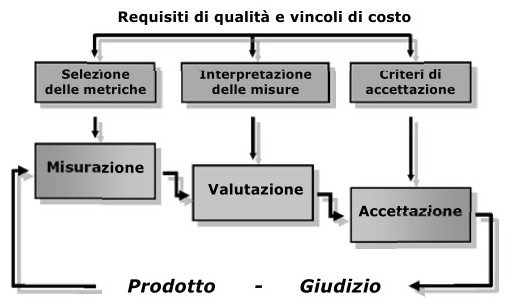
\includegraphics[width=10cm]{processo_valutazione.jpg}\\
		 Ottengo i valori, interpreto i valori e controllo se superano un valore di soglia\\
		 Processo che deve essere fatto in automatico prima del push per ogni parte
		 
		 \clearpage
		 \section{Qualità di processo}
		
		\textbf{Qualità di processo}\\
		Quality assurance, sistematico, per avere risultati riproducibili, identificando i momenti di verifica\\
		Usando PDCA, disposizione al miglioramento\\
		Ogni processo deve avere un controllo, non passivo, che aiuta a fissare obbiettivi metrici\\
		
		\textbf{Standard}\\
		ISO 9000: fondamenti e glossario\\
		ISO 9001: sistema [gestione] qualità - requisiti\\
		ISO 90003: come applicare il 9001 al SW\\
		ISO 9004: guida al miglioramento dei risultati\\
		
		\textbf{ISO 9000}\\
		Generale per qualsiasi ambito\\
		4 tipi di processi: direzione dell'azienda; gestione risorse; realizzazione del prodotto; misura, analisi e miglioramento\\
		La qualità (reparto qualità) deve essere sotto alla direzione, perché influente e consapevole, riferisce direttamente alla direzione.\\
		
		\textbf{Documentazione}\\
		-Manuale della qualità: documento trasversale, determinato dalla politica della qualità dell'azienda, univoca, definisce il sistema di gestione della qualità dell'organizzazione\\
		-Piano della qualità: documento verticale, uno per ogni progetto, definisce way of working, obbiettivi di qualità, misure e soglie di accettazione\\
		
		\textbf{Strumenti di valutazione}\\
		Per la misurazione della maturazione dei processi\\
		-SPY: valutazione oggettiva per valutare i fornitori in base alla maturità dei processi, non standardizzato\\
		-CMMI (Capability Maturity Model + Integration): strumento di valutazione dei processi dei fornitori sviluppato dal DoD\\
		-SPICE: ISO 15504 = SPY + ISO 12207 + ISO 9001\\
		
		\textbf{CMMI}\\
		-Capability: misura di adeguatezza di \textit{un processo} rispetto agli scopi assegnati, determina efficienza ed efficacia raggiungibili\\
		-Maturity: valore minimo (bottom) della capability, misura di quanto e quanto bene l'azienda è governata dal suo \textit{sistema di processi}, misura l'effetto combinato delle capability\\
		-Model: modello, insieme di criteri per valutare (in scala assoluta)\\
		-Integration: Architettura di integrazione con altre discipline (HW, SW, system) e tipologie di attività\\
		
		\textbf{Bassa capability - da evitare}\\
		Il processo ha bassa capability se:\\
		-definito e attuato in modo opportunistico\\
		-non eseguito in modo disciplinato, sistematico e quantificabile\\
		-difficile prevedere esito, avanzamento e qualità\\
		-porta a compromessi tra funzionalità e qualità\\
		
		\textbf{Governance}\\
		Diverso da managemente, visione del punto di arrivo e si procede in quella direzione\\
		
		\textbf{I 5 livelli di maturità}\\
		1 - So solo cosa devo ottenere, ma improvviso, processo imprevedibile, poco controllato, reattivo\\
		2 - D - So cosa fare, ma non come andrà, processo caratterizzato per progetti e reattivo\\
		3 - P - Ho un piano ad occhio, non ho calcolato come andrà, processo caratterizzato da una organizzazione, proattivo\\
		4 - PC - Ho un piano e so prevedere l'avanzamento (misurabile), processo misurabile e controllabile, posso gestirlo quantitativamente\\
		5 - PDCA - Ho un piano, so prevedere l'avanzamento e monitoro costantemente per migliorare, si punta al miglioramento\\
		
\end{document}
